\documentclass[10pt]{article}

%%%%%%%%%%%%%%%%%%%%%%%%%%%%%%%%%%%%%%%%%%%%%%%%%%%%%%%%%%%%%%%%%%%%%%%%%%%%%%%
%%% packages %%%
%%%%%%%%%%%%%%%%%%%%%%%%%%%%%%%%%%%%%%%%%%%%%%%%%%%%%%%%%%%%%%%%%%%%%%%%%%%%%%%

\usepackage[english]{babel} % Choose english language
\usepackage[labelfont = bf, font = small]{caption} % Use caption package. Use bold font for caption.
\usepackage{siunitx} % Use siunitx for unit representation.
\newcommand{\RM}[1]{\MakeUppercase{\romannumeral #1{:}}}
\usepackage{graphicx}
\usepackage{tabularx}
\usepackage{float}
\usepackage{lmodern}
\usepackage{filecontents}
\usepackage{amsmath}
\usepackage{amssymb}
\usepackage[utf8]{inputenc}
\usepackage[bottom]{footmisc}
\usepackage{leftidx}
\usepackage{subcaption}
\usepackage[explicit]{titlesec}
\usepackage{booktabs}
\usepackage{multirow}
\usepackage{multicol}
\usepackage{listings}
\usepackage{pgfplots}
\usepackage{natbib}
\usepackage{xcolor}
\usepackage{url}
\usepackage{array}
\usepackage{setspace}
\usepackage{hyperref} % Referencing
\usepackage{verbatim}
\usepackage{changepage}
\usepackage[footnote, printonlyused]{acronym}
\usepackage{scrextend}
\usepackage{geometry} % Change geometry of page layout
\usepackage{rotating}
\usepackage{longtable}
\usepackage{lscape}
\usepackage{tocloft}
\usepackage{tkz-euclide}
\usepackage{listings}
\usepackage{feynmp-auto} % Create fenynman diagrams
\usepackage{tikz-feynman} % Create fenynman diagrams
\usepackage{lipsum} % For testing. insert random text

%%%%%%%%%%%%%%%%%%%%%%%%%%%%%%%%%%%%%%%%%%%%%%%%%%%%%%%%%%%%%%%%%%%%%%%%%%%%%%%
%%% new commands and environments %%%
%%%%%%%%%%%%%%%%%%%%%%%%%%%%%%%%%%%%%%%%%%%%%%%%%%%%%%%%%%%%%%%%%%%%%%%%%%%%%%%

% Create custom font
\newenvironment{myfont}{\fontfamily{put}\selectfont}{\par}

% Adapt spacing between lines
\doublespacing

% Delete dots from toc
\renewcommand{\cftdot}{}

% Change section label to roman
\renewcommand{\thesection}{\Roman{section}}

% Customize section layout
\newcommand{\ssection}[1]{%
  \section[#1]{\centering\normalfont\scshape #1}}
\newcommand{\ssubsection}[1]{%
  \subsection[#1]{\centering\normalfont\itshape #1}}
\newcommand{\ssubsubsection}[1]{%
  \subsubsection[#1]{\centering\normalfont #1}}

% Import tikz libraries for figures
\usetikzlibrary{positioning,shadows,arrows}

% Create footnotereferencing
\makeatletter
\newcommand\footnoteref[1]{\protected@xdef\@thefnmark{\ref{#1}}\@footnotemark}
\makeatother

% Change layout of page
\hypersetup{
  colorlinks = true,
  linkbordercolor = {red},
  citebordercolor = {red},
  menubordercolor = {blue},
  urlbordercolor = {blue},
  linktoc = {page},
  pagebackref = {True},
  pdftitle = {Solution 06},
  pdfauthor = {Nils Hoyer, Maurice Morgenthaler},
  pdfcreator  = {pdflatex},
  pdfproducer = {LaTeX}
}

% Change geometry of page
\geometry{a4paper, top = 20mm, left = 20mm, right = 20mm, bottom = 15mm, headsep = 8mm, footskip = 10mm, includeheadfoot}

% Decalre uits for SIunitx
\DeclareSIUnit\femtobarn{fb^{-1}}
\DeclareSIUnit\percent{\%}

% Define colors
\definecolor{deepblue}{rgb}{0,0,0.5}
\definecolor{deepred}{rgb}{0.6,0,0}
\definecolor{deepgreen}{rgb}{0,0.6,0.2}
\definecolor{deeporange}{rgb}{0.9,0.2,0}

%%%%%%%%%%%%%%%%%%%%%%%%%%%%%%%%%%%%%%%%%%%%%%%%%%%%%%%%%%%%%%%%%%%%%%%%%%%%%%%
%%% start document %%%
%%%%%%%%%%%%%%%%%%%%%%%%%%%%%%%%%%%%%%%%%%%%%%%%%%%%%%%%%%%%%%%%%%%%%%%%%%%%%%%

\begin{document}
\begin{myfont}
\lstset{language=C++,
  basicstyle=\ttfamily,
  keywordstyle=\color{blue}\ttfamily,
  stringstyle=\color{red}\ttfamily,
  commentstyle=\color{green}\ttfamily,
  morecomment=[l][\color{magenta}]{\#}
}

\begin{center}
  \begin{Large}
    \textsc{Solution for homework assignment no. 06} \\
  \end{Large}
	\vspace*{0.4cm}
    Nils Hoyer, Maurice Morgenthaler
  \vspace*{1cm}
\end{center}

\section*{Exercise 6.1}

We are asked to derive the extenden likelihood function for the binned case. \\

\noindent We start by looking at the content in each bin, i.e.

\begin{equation}
n_{b}(\theta) = n_{\textrm{tot}} \int\limits_{x_{0} + h(b-1)}^{x_{0} + hb} \textrm{d}x \,\cdot\, f(x \,|\, \theta)
\end{equation}

\noindent where $h$ is the width of the bin and $b$ the bin number. \\
For a Poissonian distribtion we then get

\begin{equation}
f(m, n(\theta)) = \frac{n_{tot}^{m}e^{-n_{tot}}}{m_{tot}!} \cdot \frac{m_{tot}!}{m_{1}!\,...\, m_{N}!} \left(\frac{n_{1}}{n_{tot}}\right)^{m_{1}} \,...\, \left(\frac{n_{N}}{n_{tot}}\right)^{m_{N}} = \prod_{i = 1}^{N}\frac{n_{i}^{m_{i}}}{m_{i}!}e^{-n_{i}}
\end{equation}

\noindent Therefore

\begin{equation}
\mathcal{L} = \textrm{ln}\left(\sum_{i = 1}^{N} f(m, n(\theta)\right) = \sum_{i = 1}^{N}m_{i}\cdot \textrm{ln} \left(n_{i}\right) - \textrm{ln}\left(m_{i}\,!\right) - n_{i} \approx \sum_{i = 1}^{N}m_{i} \,\cdot\, \left(\textrm{ln}(n_{i}) - \textrm{ln}(m_{i})\right) - (m_{i} + n_{i})
\end{equation}

\noindent where I used Stirling's formula.


\section*{Exercise 6.2}

\noindent Given a PDF 

\begin{equation}
f(t\, | \, \tau) = \frac{e^{-t/\tau}}{\tau}
\end{equation}

\noindent we are asked to generate \num{100} pseudo events for $\tau_{\textrm{true}} =$ \SI{1.0}{\second}.
Using the unbinned maximum likelihood function we are asked to find the best fit value for $\tau$ by computing a local minimum using Minuit.
Afterwards we should repeat this process for the binned case with $\Delta t =$ \SI{0.5}{\second} where

\begin{equation}
\nu_{i}(\tau) = n_{\textrm{tot}} \int\limits_{t_{i}^{\textrm{min}}}^{t_{i}^{\textrm{max}}} \textrm{d}t \cdot f(t\, | \, \tau).
\end{equation}

\noindent Eventually we shall use different binning values and see what happens if $\Delta t \rightarrow $ \num{0} and $\Delta t \rightarrow \infty$. \\

\noindent The resulting plot for the randomly generated values of the exponential function and the overlying function with the fitted value for $\tau$ is shown in figure \ref{fig:ex6_2}.

\begin{figure}[H]
	\centering
	\caption{The plot shows the distribution of randomly generated values $x$ following a exponential distribution with $\tau =$ \num{1.0}.
	The overlying function shows the exponential function together with $\tau$ given by Minuit.}
	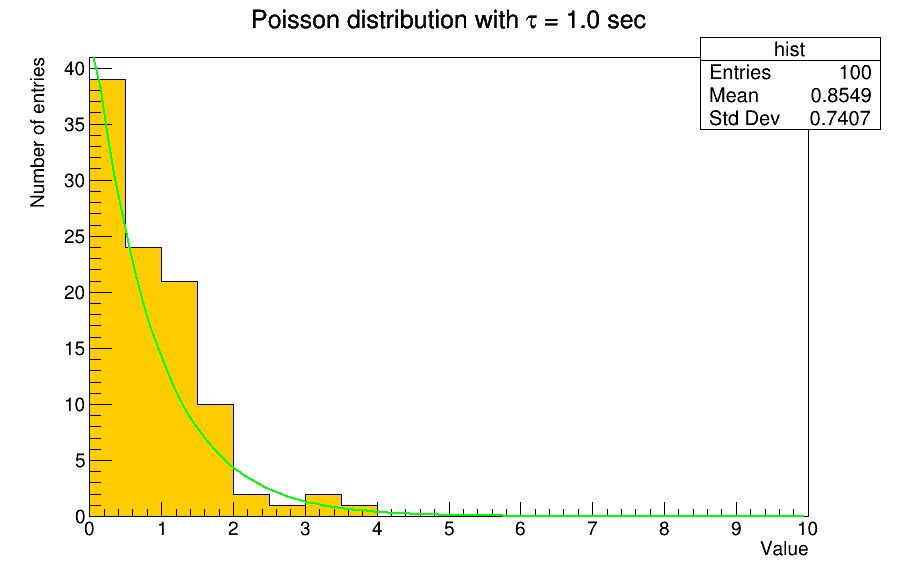
\includegraphics[width = \textwidth]{exercise6_2.png}
	\label{fig:ex6_2}
\end{figure}

\end{myfont}
\end{document}